
\documentclass{jtetiproposalskripsi}

%-----------------------------------------------------------------
%Disini awal masukan untuk data proposal tugas akhir
%-----------------------------------------------------------------
\titleind{PERANCANGAN WEB PENDAFTARAN ANGGOTA ALUMNI DI 
SMA MUHAMMADIYAH 3 JEMBER}
\fullname{TRI HENDRA JUNIARTO}

\idnum{1200631012}

\approvaldate{13 November 2013}

\degree{Sarjana Teknik Elektro}

\yearsubmit{2015}

\program{Manajemen Informatika}

\headprogram{Sarjiya, S.T., M.T., Ph.D.}

\dept{}

\firstsupervisor{Triawan Adi Cahyanto,M.Kom}
\firstnip{12 03 719}

\secondsupervisor{Bagus Setya Rintyarna,S.T,M.Kom}
\secondnip{09 03 521}


%-----------------------------------------------------------------
%Disini akhir masukan untuk data proposal skripsi
%-----------------------------------------------------------------

\begin{document}

\cover

\approvalpage

%-----------------------------------------------------------------
%Disini akhir masukan untuk muka skripsi
%-----------------------------------------------------------------

%-----------------------------------------------------------------
%Disini awal masukan Intisari
%-----------------------------------------------------------------
\begin{abstractind}
Tugas akhir ini merupakan hasil dari penelitian yang penulis lakukan pada SMA Muhammadiyah 3 Jember Melihat perkembangan tersebut kami mempunyai gagasan untuk membuat Website tentang Alumni di karenakan belum tersedianya website Alumni pada SMP N 4 Metro sehingga penulis ingin mempermudah para alumni untuk ber komunikasi dan mencari data Alumni.
Website ini di kembangkan dengan menggunakan softwere Adobe Sublime Tex 2, php mysql , website ini berisi tentang visi dan misi, struktur sekolah, sejarah sekolah,  pendaftaran alumni SMA Muhammadiyah 3 Jember dan bertujuan untuk  memperkenalkan SMA Muhammadiyah 3 Jember kepada masyarakat umum. Tugas akhir ini bertujuan membangun sebuah sistem informasi  berbasis web.
 
Masalah yang di hadapi dalam pembuatan website adalah sulitnya membuat desain halaman home, admin, user dikarenakan harus meng intregasikan  koding HTML, PHP, CSS dan membuat link yang menghubungkan page satu dengan yang lainya .  Susahnya membuat link untuk  untuk menyimpan ke database supaya data yang di inputkan bisa  masuk kedatabase.
 
Dengan demikian sistem ini diharapkan dapat mempermudah kerja staff, Guru karena  tidak perlu melakukan pencarian melalui arsip sekolah kita hanya perlu buka data base lalu ekport. Website Alumni  SMA Muhammadiyah 3 Jember merupakan sarana informasi online yang dapat di akses oleh siapun maupun  masyarakat umum untuk mengetahui informasi tentang sekolah .  sebagai forum diskusi atau komunikasi antara alumni satu dengan yang lainya dan  mencari data para alumni SMA Muhammadiyah 3 Jember.



\bigskip

\end{abstractind}
%-----------------------------------------------------------------
%Disini akhir masukan Intisari
%-----------------------------------------------------------------

\tableofcontents
\addcontentsline{toc}{chapter}{DAFTAR ISI}
\selectlanguage{bahasa}\clearpage\pagenumbering{arabic}\setcounter{page}{1}

%-----------------------------------------------------------------
%Disini awal masukan untuk Bab
%-----------------------------------------------------------------
\chapter{LATAR BELAKANG}

\section{Latar Belakang Masalah}
Teknologi dan informasi merupakan dua hal yang tidak dapat dipisahkan, hal ini terlihat dari proses mendapatkan informasi yang dapat diperoleh secara cepat, tepat dan akurat dengan dukungan teknolgi yang semakin canggih. Kemajuan teknologi ini membuat banyak organisasi dan lembaga pendidikan menggunakan teknologi berbasis komputer dan jaringan untuk membantu untuk membantu pekerjaannya karena bersifaat efektif dn efisien. 

Banyak lembaga pendidikan yang telah menggunakan sistem terkomputerisasi dalam pengolahan datanya. SMA Muhammadiyah 3 Jember adalah sebuah lembaga pendidikan menengah atas yang berada di Kabupaten Jember, sekolah swasta yang sudah dikenal oleh masyarakat khusunya daerah Jember. Disisi lain penyampaian informasi mengenai profil dari SMA Muhammadiyah sendiri hanya dapat diterima oleh masyarakat di sekitarnya saja, ketika masyarakat luar ingin mengakses untuk mendapatkan informasi tentang SMA Muhammadiyah 3 Jember sangatlah sulit. Dan juga proses pendaftaran alumni hingga pencarian data alumni yang masih kurang efektif.

Dari anaslisa tersebut dapat diambil solusi mengenai suatu pengembangan Website yang akan diterapkan di SMA Muhammadiyah 3 Jember, WEB tersebut nantinya akan menjadi sebuah sumber informasi bagi masyarakat luar, yang  berisi Profil SMA Muhammadiyah 3 Jember, Visi dan Misi, Sruktur Organisasi, dan pendaftaran Alumni .Dengan dibangunya Website ini diharapkan agar masyarakat luas dapat mengakses mengenai profil SMA Muhammadiyah 3 Jember dengan mudah,proses pencarian alumni juga mudah dilakukan dan meminimalisir terjadinya datan yang hilang atau rusak. Oleh karena itu penulis membuat penelitian tugas akhir dengan judul  PERANCANGAN WEB PENDAFTARAN ANGGOTA ALUMNI SEKOLAH PADA SMA MUHAMMADIYAH 3 JEMBER .
.

\section{Rumusan Masalah}
Berdasarkan latar belakang di atas terdapat masalahyang dihadapi, Adapun masalah yang dihadapi setelah melakukan analisa adalah sebagai berikut:

1.	Proses pencarian data alumni yang kurang efisien.

2.	Proses pendaftaran alumni sekolah yang kuran efektif.

3.	Tejadinya kerusakan dan hilangnya data alumni.

4.	Kurang mengenalnya masyarakat luar terhadap SMA Muhammadiyah 3 Jember

\section{Batasan Masalah}
Penelitian ini memiliki batasan ruang lingkup penelitian ,yang meliputi:

1.	Perangan Website yang meliputi proses pendaftaran alumni sekolah .

2.	Website yang dibangun berisikan informasi mengenai profil sekolah seperti: Visi dan Misi, Struktur organisasi, sejarah skolah dan Data alumni sekolah.

3.	Perancangan ini hanya digunakan di SMA Muhamadiyah 3 Jember .


\section{Tujuan Penelitian}
Tujuan dibangunya sebuah Website ini yaitu dijabarkan sebagai beriku:

1.	Agar memudahkan masyarakat luar untuk mendapatkan informasi tentang SMA Muhammadiyah 3 Jember.

2.	Agar proses penginputan dan pencarian data alumni SMA Muhammadiyah 3 Jember menjadi lebih mudah.

3.	Meminimalisir Agar data yang para alumni tetap utuh , tidak hilang ataupun rusak  .

\section{Manfaat Penelitian}
 Manfaat yang diharapkan nantinya  nantinya setelah pembuatan Website ,adalah sebagai beriku:

1.	Bagi masyarakat luar, dapat mengakses dan mendapatkan informasi mengenai SMA Muhammadiyah 3 Jember dengan mudah.

2.	Bagi SMA Muhammadiyah 3 Jember, dapat dikenal oleh masyarakat luas melalui Website .

3.	Memudahkan staff dalam proses pencarian daftar alumni sekolah secara cepat tepat dan akurat.

4.	Manfaat bagi penulis agar dapat memenuhi syarat tugas akhir .


\section{Metodelogi Penelitian}
Metode yang diterapkan dalam pencarian data meliputi dua macam metode yakni :

1.	Metode Observasi Secara Langsung
Metode observasi ini dilakukan dengan melihat proses kerja yang terjadi di lapangan yakni di lingkungan kerja SMA Muhammadiyah 3 Jember.

2.	Metode Wawancara
Metode ini digunakan untuk mengetahui permasalahan maupun proses kerja yang terjadi di instansi. Dengan narasumber yang berkompeten sehingga didapatkan data-data yang akurat. Hal ini dapat mempermudah melakukan proses analisis permasalahan.
.

\section{Sistematika Penulisan}
Uraian singkat mengenai struktur penulisan pada masing-masing bab adalah sebagai berikut:

\textbf {BAB I PENDAHULUAN}
Membahas Latar Belakang Masalah, Identifikasi Masalah, Batasan Masalah, Tujuan Penelitian, Metodelogi Penelitian serta Sistematika Penulisan.

\textbf {BAB II LANDASAN TEORI}
Memaparkan teori-teori yang didapat dari sumber-sumber yang relevan untuk digunakan sebagai panduan dalam penelitian serta penyusunan laporan tugas akhir.

\textbf {BAB III METODOLOGI PENELITIAN}
Berisi tentang perancangan sistem serta komponen-komponen pemodelan sistem yang digunakan.

\textbf {BAB IV PENUTUP}
Mengemukakan kesimpulan yang diambil dari hasil penelitian dan perancangan sistem, serta saran-saran untuk pengembangan selanjutnya, agar dapat dilakukan perbaikan-perbaikan di masa yang akan datang.



%-------------------------------------------------------------------------------
\chapter{TINJAUAN PUSTAKA DAN DASAR TEORI}                

\section{Tinjauan Pustaka}
Tinjauan Pustaka laporan penelitian yang dijadikan referensi dalam Tugas Akhir ini adalah Tugas Akhir yang disusun oleh Tri Hendra J. (1200631012) jurusan Manajemen Informatika Universitas Muhammadiyah Jember PERANCANGAN WEB PENDAFTARAN ANGGOTA ALUMNI SEKOLAH PADA SMA MUHAMMADIYAH 3 JEMBER. Sistem tersebut disusun menggunakan bahasa pemrograman PHP  dan menggunakan database MySQL.

\section{Landasan Teori}
\subsection{Pengertian Web}
Menurut Al-Bahra bin Ladjamudin Word Wide Web (WWW), lebih dikenal dengan web,yang merupakan salah satu layanan yang didapat oleh pemakaian komputer yang terhubung ke Internet. Web pada awalnya ruang informasi dalam internet , denagn menggunakan Hypertext, pemakai dituntut untuk dapat menemukan informasi dengan mngikuti link yang disediakan web yang ditampilkan dalam Browser web.

Kini internet identic dengan web, karena kepopuleran web sebagai standar interface pada layanan  layanan yang ada di internet , dari awalnya sebagai penyedia layanan informasi, kini digunakan untuk komunikasi dari email sampai chating, sampai dengan melakukan transaksi (e-commerce) .web memudahkan pengguna komputer untuk berinteraksi dengan pelaku Internet lainya dan menelusuri informasi di internet.

\subsection{Pengertian Web Server}
Menurut Andry SyahPutra (2003 : 1), Web Server merupakan suatu 
server internet yang menggunakan protokol HTTP (Hypertext Transfer Protocol) 
untuk melayani semua proses pentransferan data.  
Sebuah komputer yang berada pada sebuah jaringan akan memiliki 
sebuah alamat yang unik, demikian pula dengan sebuah situs web pada internet. 
Situs tersebut akan memiliki alamat yang unik juga. Aktivitas utama yang 
berlangsung di internet adalah pengiriman/penerimaan e-mail dan pencarian 
informasi yang telah disediakan oleh Web Server atau sering kita sebut browsing 
atau surfing.

\subsection{Web Server}
Web server dapat mengacu pada perangkat keras atau perangkat lunak yang membantu dalam penyampaian konten web yang dapat diakses melalui internet.
Penggunaan web server yang paling umum adalah sebagai host untuk halaman web, walaupun ada beberapa penggunaan lain seperti game, media penyimpan data, atau penjalanan aplikasi perusahaan.

\subsection{Pengertian PHP}
Menurut Didik Dwi Presetyo (2004 : 76), PHP merupakan bahasa 
scripting server-side, dimana pemrosesan datanya dilakukan pada sisi server. 
Sederhananya, serverlah yang akan menerjemahkan skrip program, baru 
kemudian hasilnya akan dikirim kepada client yang melakukan permintaan.

\subsection{Keunggulan PHP}
Seluruh aplikasi berbasis web dapat dibuat dengan PHP. Namun 
kekuatan yang paling utama PHP adalah pada konektivitasnya dengan sistem 
database di dalam web. Kelebihan-kelebihan dari PHP diantaranya adalah : 

a. PHP mudah dibuat dan dijalankan, maksudnya PHP dapat berjalan 
    dalam Web Server dan dalam Sistem Operasi yang berbeda pula. 

b. PHP adalah software open-source yang gratis dan bebas didistribusikan 
    kembali di bawah lisensi GPL (GNU Public License). User dapat men
   download kode-kode PHP tanpa harus mengeluarkan uang atau khawatir 
   dituntut oleh pihak pencipta PHP. 

c. PHP bisa dioperasikan pada platform Linux ataupun Windows. 

d. PHP sangat efisien, karena PHP hanya memerlukan resource system 
    yang sangat sedikit dibanding dengan bahasa pemograman lain. 

e. Ada banyak Web Server yang mendukung PHP, seperti Apache, PWS, 
    IIS, dan lain-lain. 

f. PHP juga didukung oleh banyak database, seperti MySQL, PostgreSQL, 
   Interbase, SQL, dan lain-lain. 

g. Bahasa pemograman PHP sintaknya sederhana, singkat dan mudah 
    untuk dipahami. 

h. HTML-embedded, artinya PHP adalah bahasa yang dapat ditulis dengan 
menempelkan pada sintak-sintak HTML

\subsection{Pengertian Mysql}
Menurut Didik Dwi Prasetyo (2004 :18) MySQL merupakan salah satu 
database server yang berkembang di lingkungan open source dan didistribusikan 
secara free (gratis) dibawah lisensi GPL. 
MySQL merupakan RDBMS (Relational Database Management 
System) server. RDBMS adalah program yang memungkinkan pengguna database 
untuk membuat, mengelola, dan menggunakan data pada suatu model relational. 
Dengan demikian, tabel-tabel yang ada pada database memiliki relasi antara satu 
tabel dengan tabel lainnya.

\subsection{Keunggulan Mysql}
Beberapa keunggulan dari MySQL yaitu : 
a. Cepat, handal dan Mudah dalam penggunaannya 
MySQL lebih cepat tiga sampai empat kali dari pada database server 
komersial yang beredar saat ini, mudah diatur dan tidak memerlukan 
seseorang yang ahli untuk mengatur administrasi pemasangan MySQL. 

b. Didukung oleh berbagai bahasa 
Database server MySQL dapat memberikan pesan error dalam berbagai bahasa seperti Belanda, Portugis, Spanyol, Inggris, Perancis, Jerman, dan Italia. 

c. Mampu membuat tabel berukuran sangat besar 
Ukuran maksimal dari setiap tabel yang dapat dibuat dengan MySQL 
adalah 4 GB sampai dengan ukuran file yang dapat ditangani oleh sistem operasi yang dipakai. 

d. Lebih Murah 
MySQL bersifat open source dan didistribusikan dengan gratis tanpa 
biaya untuk UNIX platform, OS/2 dan Windows platform.  

e. Melekatnya integrasi PHP dengan MySQL 
Keterikatan antara PHP dengan MySQL yang sama-sama software open source sangat kuat, sehingga koneksi yang terjadi lebih cepat jika 
dibandingkan dengan menggunakan database server lainnya. Modul 
MySQL di PHP telah dibuat built-in sehingga tidak memerlukan 
konfigurasi tambahan pada file konfigurasi php.ini.



%-------------------------------------------------------------------------------
\chapter{METODOLOGI}

\section{Alat dan Bahan}
Bahan dan Alat yang digunakan dalam pembuatan Website berupa Software dn Hardware ,adalah sebagai berikut:

\vspace{-0.5cm}

\begin{enumerate}[a.]
\begin{singlespace}
\itemsep0em
\item Laptop.
\item Sublime Text2 editor script PHP.
\item XAMPP sebagai web server.
\item Browser menjalankan aplikasi berbasis web.

\end{singlespace}
\end{enumerate}

\section{Langkah Kerja}
Langkah-langkah yang akan dikerjakan dalam proses pembuatan website, yang akan di paparkan sebagai berikut:

1.	Analisis Kebutuhan 

Menutut Yogia Yanto (1995) Analisis sistem adalah mengidentifikasi, mempelajari masalah-masalah yang timbul dan menentukan kebutuhan pemakaian sistem. Dengan menganalisis dapat ditentukan apa saja yang harus diterapkan pada sistem yang akan dibangun, agar sesuai dengan kebutuhan yang diinginkan user.

2.	Desain Sistem

Proses desain akan menerjemahkan syarat kebutuhan ke sebuah perancangan perangkat lunak sebelum dibuat coding. Proses ini  berfokus pada : struktur data, arsitektur perangkat lunak, representasi interface, dan detail algoritma procedural. Tahapan akan menghasilkan dokumen yang disebut software requirment dokumen ini yang akan digunakan programmer untuk melakukan aktifitas pembuatan sistemnya.

3.	Pengkodingan dan Testing

Coding merupakan penerjemahan design dalam bahasa yang bisa dikenali oleh komputer . dilakukan oleh programmer yang akan menterjemahkan transaksi yang diminta oleh user. Tahapan inilah yang merupakan tahapan secara nyata dalam mengerjakan suatu sistem. Dalam artian penggunaan komputer akan dimaksimalkan. Setelah pengkodingan selesai maka akan dilakukan tahapan testing terhadap sistem yang telah dibuat tadi. Tujuannya adalah menemukan kesalahan-kesalahan terhadap sistem tersebut dan kemudian bisa diperbaiki.

4.	Penerapan

Tahapa final setelah kita melakukan analisa, desain dan pengkodean, maka sistem yang sudah jadi akan digunakan oleh user.

5.	Pemeliharaan

Perangkat lunak yang sudah disampaikan kepada pelanggan pasti  akan mengalami perubahan. Perubahan tersebut bisa karena megalami kesalahan karena perangkat lunak harus menyesuaikan lingkungan baru, atau karena pelanggan memerlukan perkembangan fungsional.



\section{Jadwal Kegiatan}
Penelitian direncanakan akan dilaksanakan selama enam bulan. Rincian rencana jadwal penelitian dicantumkan dalam tabel berikut.

\begin{center}
Tabel 3.1. Jadwal Penelitian.
\end{center}
\vspace{-0.5cm}
\begin{figure}[ht!]
  \centering
    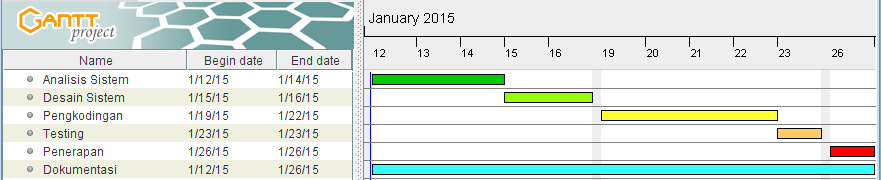
\includegraphics[width=13cm]{gambar/jadwal}

\end{figure}

%-----------------------------------------------------------------
%Disini akhir masukan Bab
%-----------------------------------------------------------------

%-----------------------------------------------------------------
%Disini awal masukan untuk Daftar Pustaka
%-----------------------------------------------------------------
%%\nocite{Abel2010,Guerbas201350}
%%\bibliography{research-plan}
%%\bibliographystyle{plainnat}
\begin{thebibliography}{9}

\bibitem[satu(2013)]{satu01}
Andi Kristanto 2008:1. Perancangan Sistem Informasi dan Aplikasinya,  

\bibitem[dua(2013)]{dua02}
Abdul Kadir .2008. MySQL (baca: mai-se-kyu-el) merupakan software yang tergolong sebagai DBMS (Database Management System) yang bersifat Open Source. 

\bibitem[tiga(2013)]{tiga03}
Abdul Kadir .2008.  PHP merupakan bahasa pemrograman berbentuk script yang ditempatkan dalam server dan diproses di server 

\bibitem[empat(2013)]{empat04}
Drs. Zulkifli Amsyah (2001:27) Pengertian Sistem  

\bibitem[lima(2013)]{lima05}
Hartono Jugiyanto  .2001. Analisis dan Disain. , C.V Andi Offset, Yogyakarta

\bibitem[enam(2013)]{enam06}
Ramadhan, Arief. 2006. Pemrograman Web Database dengan PHP dan MySQL.

\bibitem[tujuh(2013)]{tujuh07}
http://id.wikipedia.org/wiki/HTML. Diakses tanggal 9 Januari 2015

\bibitem[tujuh(2013)]{tujuh08}
http://id.wikipedia.org/wiki/Internet. Diakses tanggal 9 Januari 2015

\bibitem[tujuh(2013)]{tujuh09}
http://id.wikipedia.org/wiki/MYSQL. Diakses tanggal 9 Januari 2015

\end{thebibliography}
\addcontentsline{toc}{chapter}{DAFTAR PUSTAKA}
%-----------------------------------------------------------------
%Disini akhir masukan Daftar Pustaka
%-----------------------------------------------------------------

\end{document}